%Tema para beamer "CCM3" versión 1
%Desarrollo por Erick David Luna Núñez y 
%Fernanda Barajas Hernandez

\documentclass{beamer}

\usepackage[utf8]{inputenc}
% \usepackage{heuristica}
\usepackage[T1]{fontenc}
% \usepackage[heuristica,vvarbb,bigdelims]{newtxmath}
\renewcommand*\oldstylenums[1]{\textosf{#1}}
% \usepackage[sfdefault,scaled=.85]{FiraSans}
\usepackage{graphicx}
% \usepackage[spanish]{babel} 
\usepackage[pages=some]{background}
\pagenumbering{arabic}



%%Se define el "environment" teorema
\newtheorem{cuadro}{Objetivos del tema}
\newtheorem{cuadro2}{Objetivos de la clase}

%Definir el autor con el estilo definido (el textbf y el uso del color son herramientas del diseño, no necesario borrar)
\title{ \textbf{Álgebra I} \\ {\color{mostazaccm}\Large Clase metodológica}}

%Nombre del autor
\author{Amanda Cordero Lezcano\\
        Christopher Guerra Herrero} 

%Fecha o evento en que se presentará la plática
\date{Festival de la clase, Mayo 2023} 

%correo del expositor o incluir posibles colaboradores
\institute{Tutora: MSc. Celia Tamara González González\\
Facultad de Matemática y Computación} 


%%Tema de beamer "CCM-3"
\usetheme{ccm3}

\begin{document}
%Define el fondo de la primer diapositiva
{\setbeamertemplate{background}{
  
\includegraphics[width=\the\paperwidth,height=\the\paperheight]{images/P3.png}}
%lo anterior es para definir el fondo de la primer diapositiva

\begin{frame}
  \titlepage %Necesario para generar la portada
\end{frame}

} %aquí termina el cambio de fondo

\begin{frame}

  \begin{itemize}
    \item[\checkmark] {\Large Disciplina: Matemática Básica}
    \item[\checkmark] {\Large Álgebra I para 1er Año de Licenciatura en Ciencia de la Computación}
    \item[\checkmark] {\Large Tema III: Sistemas de Ecuaciones Lineales}
    \item[\checkmark] {\Large Clase práctica: Método de Gauss}
  \end{itemize}

\end{frame}

\begin{frame}
  \tableofcontents %Imprime la tabla de contenido
\end{frame}

\section{Objetivos del ejercicio} %%Título de la sección (Opcional)
\begin{frame}
  \frametitle{I. Objetivo general}
  \begin{itemize}
    \item Establecer correctamente la relación entre el saber matemático y la realidad objetiva,
          entre el modelo matemático y la realidad modelada
    \item Desarrollar las habilidades para el trabajo independiente, la constancia y la organización del estudio.
    \item Potenciar acciones encaminadas al uso de softwares específicos de su campo profesional
  \end{itemize}
\end{frame}

\section{Aspectos metodológicos}
\begin{frame}{II. Aspectos metodológicos} %%Otra forma (más corta) de poner el título a la diapositiva
  \framesubtitle{Proceso de Enseñanza Aprendizaje}
  \begin{center}
    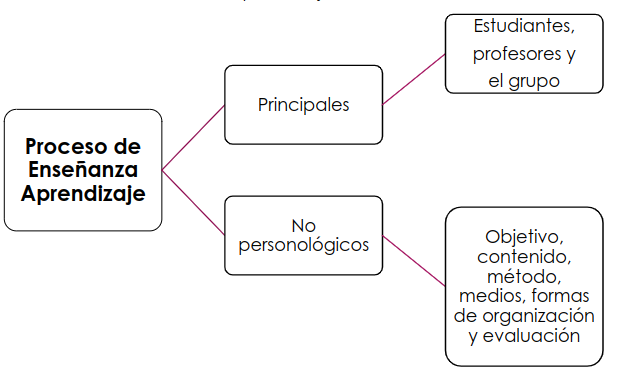
\includegraphics[width=9.0cm]{images/Grafica1.png}
  \end{center}
\end{frame}

\section{Ubicación del tema dentro del programa de la Asignatura} %%Otra sección
\begin{frame}{Unidades de la Asignatura}
  \begin{enumerate}
    \item Números Complejos
    \item Polinomios
    \item {\bf Sistemas de Ecuaciones Lineales}
    \item Espacios Vectoriales y Subespacios Vectoriales
    \item Aplicaciones Lineales
    \item Valores y Vectores Propios
  \end{enumerate}
\end{frame}

\begin{frame}{Sistemas de Ecuaciones Lineales}
  \framesubtitle{Objetivos generales del tema}
  \begin{itemize}
    \item Reconocer y diferenciar, teórica y prácticamente, las estructuras algebraicas fundamentales
          y desarrollen habilidades para el cálculo en las mismas y su aplicación a la resolución de tareas
          concretas
    \item Simplificar el trabajo con determinados entes matemáticos al trabajo con matrices,
          desarrollando habilidades para realizar tal representación del modo que más convenga al probema tratado
  \end{itemize}

\end{frame}

\section{Antecedentes y Motivación}
\begin{frame}{Antecedentes y Motivación}
  \begin{center}
    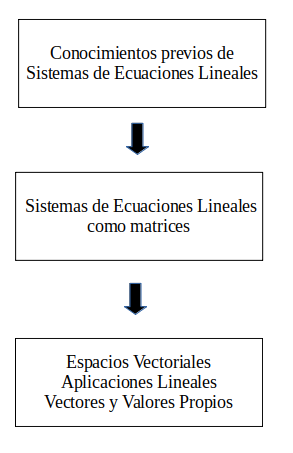
\includegraphics[width=3.5cm]{images/Grafica3.png}
  \end{center}
\end{frame}

\begin{frame}
  \framesubtitle{Desglose por horas}
  {\centering \Large Clases Conferencias: 8\\
    Clases Prácticas: 8\\
    Total: 16\\}
\end{frame}

\begin{frame}
  \begin{center}
    {\bf \Large Valores Fundamentales de la Carrera}
  \end{center}
  \begin{itemize}
    \item Desarrollar habilidades para realizar  procesos de generalización, abstracción y las formas de pensamiento lógico
    \item Utilizar los contenidos abordados en el desarrollo computacional de problemas específicos
    \item Contribuir a que los alumnos puedan establecer correctamente la relación dialéctica entre
          un modelo matemático y los fenómenos reales que este representa
  \end{itemize}

\end{frame}

\begin{frame}{Sistemas}

  \framesubtitle{Conocimientos y Habilidades}
  \begin{itemize}
    \item Representar matricialmente sistemas lineales y utilizar tal representación para clasificar y resolver sistemas
    \item Hallar ejemplos en que se verifiquen o no las condiciones que caracterizan a los diferentes conceptos y propiedades abordados en el programa de la asignatura
    \item Realizar operaciones con matrices
  \end{itemize}
\end{frame}

\begin{frame}
  \begin{cuadro2}
    Aplicar el Método de Gauss para la resolución de Sistemas de Ecuaciones Lineales, y las definiciones asociadas
    a este concepto en la resoluciónde ejercicios
  \end{cuadro2}
\end{frame}

\begin{frame}{Métodos y medios}
  \framesubtitle{}
  {\bf Métodos}
  \begin{itemize}
    \item La exposición problemática
    \item La búsqueda parcial
    \item La conversación heurística
  \end{itemize}
  {\bf Medios}
  \begin{itemize}
    \item Pizarra
    \item Dispositivos Móviles
    \item NumPy, Python
  \end{itemize}
\end{frame}


\section{Bibliografía}
\begin{frame}{Bibliografía}
  %posibles estilos para bibliografía: unsrt , siam , plain , ieeetr , alpha , acm , abbrv
  \bibliographystyle{apalike}
  \bibliography{references}
  {\bf Básica}
  \begin{itemize}
    \item Kurosch, R. Curso de Algebra Superior. Pueblo y Educación 1987
    \item Solana M. Roldán R. Apuntes para un curso de Algebra Lineal.
  \end{itemize}
  {\bf Complementaria}
  \begin{itemize}
    \item Lipschutz, S. Algebra lineal. Teoría y 600 problemas resueltos,
          edición revolucionaria
    \item Faddieev, D. Problemas de Algebra Superior. Pueblo y
          Educación 1971
  \end{itemize}
\end{frame}



\section{Asimilación y nivel de partida}
\begin{frame}{Conferencia anterior}
  La autopreparación para esta clase debió basarse en las notas de clase de las
  conferencias. Para la resolución de los ejercicios es necesario el conocimiento de la definición y
  propiedades básicas de la teoría de los Sistemas de Ecuaciones Lineales. Es importante
  recordar estos temas como introducción a la clase.
\end{frame}

\section{Ejercicios}
\subsection{Aplicación del método de Gauss}
\begin{frame}
  {Ejercicio 1} Resolver utilizando el método de Gauss:          $$2x+y+z=3$$
  $$x-2y+3z=4$$
  $$-2x+z=1$$

\end{frame}
\begin{frame}{Solución}
  $$\left(
    \begin{array}{rrrrl}
        2  & 1  & 1 & \bullet & 3 \\
        1  & -2 & 3 & \bullet & 4 \\
        -2 & 0  & 1 & \bullet & 1
      \end{array}
    \right) \sim \left(
    \begin{array}{rrrrl}
        2 & 1  & 1  & \bullet & 3  \\
        0 & -3 & -5 & \bullet & -5 \\
        0 & 1  & 2  & \bullet & 4
      \end{array}
    \right)$$
  $$\hspace*{4cm}
    \sim \left(
    \begin{array}{rrrrl}
        2 & 1  & 1  & \bullet & 3  \\
        0 & -3 & -5 & \bullet & -5 \\
        0 & 0  & 1  & \bullet & 7
      \end{array}
    \right)$$

  $$z=7$$
  $$y=0$$
  $$x=-2$$
\end{frame}
\subsection{Sistemas con parámetros}
\begin{frame}
  {Ejercicio 2} Qué condiciones deben verificar los parámetros $a$, $b$, $c$ para que el sistema:
  $$x_1 +2x_2-3x_3=a$$
  $$2x_1 +6x_2-11x_3=b$$
  $$x_1 -2x_2+7x_3=c$$
  posea alguna solución. En tal caso, cuántas soluciones posee.

\end{frame}
\begin{frame}{Solución}
  $$\left(
    \begin{array}{rrrrl}
        1 & 2  & -3  & \bullet & a \\
        2 & 6  & -11 & \bullet & b \\
        1 & -2 & 7   & \bullet & c
      \end{array}
    \right) \sim \left(
    \begin{array}{rrrrl}
        1 & 2  & -3 & \bullet & a    \\
        0 & 2  & -5 & \bullet & b-2a \\
        0 & -4 & 10 & \bullet & c-a
      \end{array}
    \right)$$
  $$\hspace*{4cm}
    \sim \left(
    \begin{array}{rrrrl}
        1 & 2 & -3 & \bullet & a         \\
        0 & 2 & -5 & \bullet & b-2a      \\
        0 & 0 & 0  & \bullet & 2b -5a +c
      \end{array}
    \right)$$

  $$0x_3=2b -5a +c$$
  $$0=2b -5a +c$$
\end{frame}
\begin{frame}{Solución}
  El sistema tendrá solución solo si $2b -5a +c=0$. En tal caso tendrá
  infinitas soluciones por ser compatible indeterminado.
\end{frame}
\begin{frame}
  {Ejercicio 3} Determinar los valores del parámetro $k$ para que el sistema
  $$x_1 -3x_3=3$$
  $$2x_1 +kx_2-x_3=2$$
  $$x_1 +2x_2+kx_3=1$$
  tenga infinitas soluciones
\end{frame}
\begin{frame}{Solución}
  $$\left(
    \begin{array}{rrrrl}
        1 & 0 & -3 & \bullet & 3 \\
        2 & k & -1 & \bullet & 2 \\
        1 & 2 & k  & \bullet & 1
      \end{array}
    \right) \sim \left(
    \begin{array}{rrrrl}
        1 & 0 & -3  & \bullet & 3  \\
        0 & k & 5   & \bullet & -4 \\
        0 & 2 & k+3 & \bullet & -2
      \end{array}
    \right)$$
  $$\hspace*{4cm}
    \sim \left(
    \begin{array}{rrcrl}
        1 & 0 & -3                  & \bullet & 3   \\
        0 & k & 5                   & \bullet & -4  \\
        0 & 0 & \frac{-k(k+3)}{2}+5 & \bullet & k-4
      \end{array}
    \right)$$
\end{frame}

\begin{frame}{Solución}
  Note que
  $$\frac{-k(k+3)}{2}+5 = \frac{-k^2-3k+10}{2}=\frac{-(k+5)(k-3)}{2}$$
  expresión que se anula si $k=-5$ o $k=3$.\\
  Pero el miembro derecho $k-4$ solo se anula cuando $k=4$.\\
  Por tanto el sistema no tendrá infinitas soluciones para ningún valor de $k$

\end{frame}

\section{Conclusiones}
\begin{frame}{Ejercicios complementarios}
  Se socializa un documento digital con mayor cantidad de ejercicios para el estudio individual.
\end{frame}
\begin{frame}{Temas a continuación}
  En los siguientes encuentros se continuará trabajando el mismo tema. Además, los conocimiento
  adquiridos serán de provecho para habilidades de las unidades próximas como
  caracterizar espacios vectoriales o hallar la matriz asociada a una aplicación lineal.
\end{frame}


{\setbeamertemplate{background}{
  
\includegraphics[width=\the\paperwidth,height=\the\paperheight]{images/P3.png}}
%lo anterior es para definir el fondo de la primer diapositiva

\begin{frame}
  \titlepage %Necesario para generar la portada
\end{frame}

}


\end{document}